% Chapter Template

\chapter{Proposed Methodology} % Main chapter title

\label{c4} % Change X to a consecutive number; for referencing this chapter elsewhere, use \ref{ChapterX}


 \section{Proposed Methodology}
 
 
 \subsection{Proposed 1: Hybrid GRU-CNN Model}
 
 
 An end-to-end DL paradigm is used,  allowing for automated ECG analysis.  GRU addresses problems with long sequences with widely separated features. GRU makes the final choice on how much of the past should be remembered and how much should be forgotten. The GRU cell receives two inputs: the previous concealed state and the current timestamp. These are combined and passed through the update and reset gates by the cell. To predict the output in the current timestep,  the hidden state must be passed via a thick layer with an activation function. As a result,  a new hidden state is obtained,  which is then passed on to the following time step. The update gate selects which current GRU cell will send data to the next GRU cell. It aids in remembering the most crucial facts. Figure \ref{Fig:5} is our proposed framework:



    \begin{figure}
      \centering
      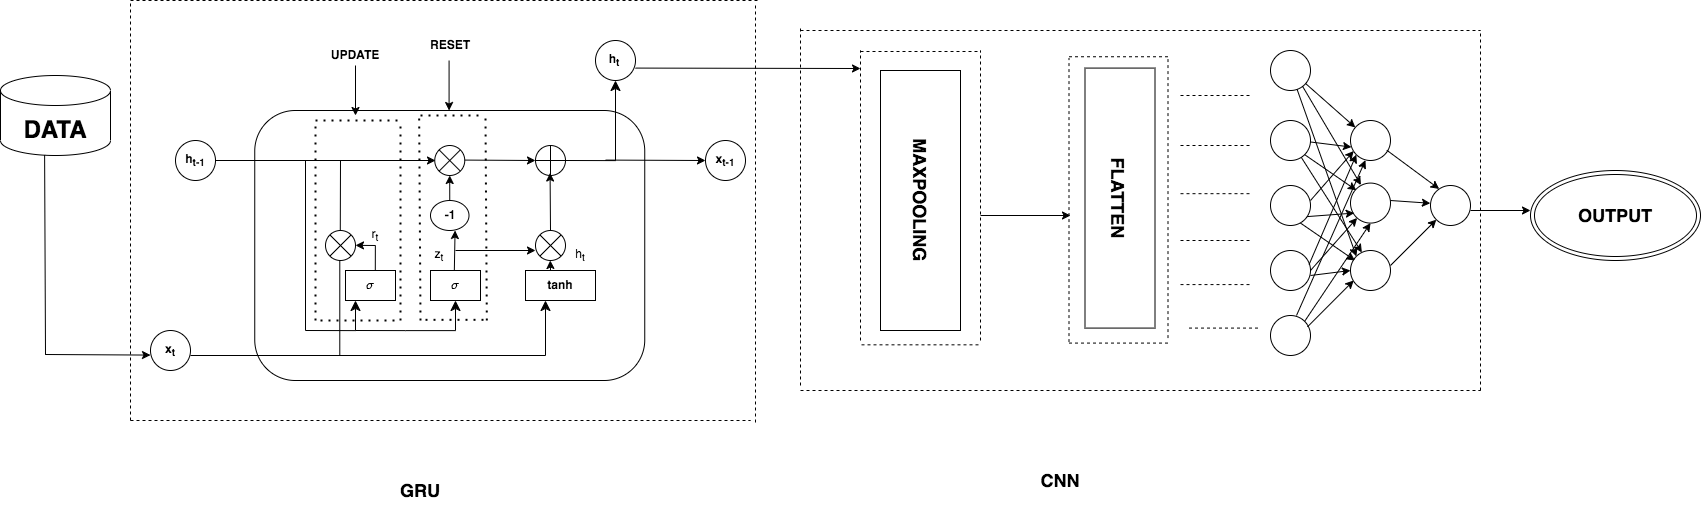
\includegraphics[scale= 0.25]{architecturepro1.png}
      \caption{Proposed hybrid GRU-CNN model framework}
      \label{Fig:5}
    \end{figure}



 Let our timeseries data be denoted as, 
 \begin{equation}
  X = [ x_1,  x_2,  x_3.... x_m]
 \end{equation}

where,   $x_t \in X$ and $[t = 1, 2, 3...m]$ ,  $t \in Z^+$ . The update gate's inputs are the hidden layer from the previous timestep $(h_{t-1})$ and the current input $( x_t )$. Both have related weights that are learned during the training phase. Let us say that the weights associated with $(h_{t-1})$ is $( U_z )$ and that of $( x_t )$ is $( W_z )$. The output of the update gate $( Z_t )$ is given by, 

\begin{equation}
  z_t = \sigma(W_z x_t + U_z h_{t-1})
\end{equation}
A reset gate identifies unnecessary information and decides what information to remove from the GRU network; in other words,  it decides what information to delete at a specific timestamp. The input to the reset gate is the hidden layer at the previous timestep $(h_{t-1})$ and the current input $( x_t )$ 
Both have related weights that are learned during the training phase.  Let us say that the weights associated with $(h_{t-1})$ is $(U_r)$ and that of  $( x_t )$ is $(W_r)$.  The output of the update gate $( r_t )$ is given by, 

\begin{equation}
  r_t = \sigma(W_r x_t + U_r h_{t-1})
\end{equation}

GRU networks interpret sequential data,  such as time series or plain language,  by avoiding the hidden state from one time step to the next. The hidden state is a vector that contains information from previous time steps that are relevant to the current time step. The primary principle behind a GRU is to let the network decide which information from the previous time step is relevant to the current time step and which may be ignored.


The reset gate is used to calculate a candidate's hidden state. This is utilised to determine the information that has been stored in the past. This is sometimes referred to as the memory component in a GRU cell. It is calculated as follows, 
\begin{equation}
  \tilde{h}_t = \tanh(W_{x_{t}} + r_t \odot U_{h_{t-1}})
\end{equation}

Here,  $W_{x_{t}}$ : Weight associated with the current input,  $r_t$ : Output of the reset gate,  $U_{h_{t-1}}$ : Weight associated with the hidden layer of the previous timestep,  $\tilde{h}_t$ : Candidate hidden state.



The new hidden state is calculated using the following formula,  which is dependent on the update gate and candidate hidden state.
\begin{equation}
  {h}_t = ( z_t \odot h_{t-1} + (1- z_t)\odot \tilde{h}_t)
\end{equation}

Here,  $z_t$ : Output of update gate,  $h_{t-1}$ : Hidden state at the previous timestep , $\tilde{h}_t$ : Candidate hidden state(Final output from GRU cell).

As the above formula,  whenever $z_t$ is 0,  the previously buried layer's information is forgotten. It is updated with the new candidate hidden layer's value (as 1- $z_t$ will be 1). If $z_t$ is 1,  the information from the previously hidden layer is then preserved. This is how the most important data is transferred from one state to the next. Now only important data is left as to pass in input for CNN. The output from GRU is fed into 1-D CNN. The Conv1D layers smooth the input time-series,  eliminating the need to include the rolling mean and rolling standard deviation values in the input features.





Maximum pooling and dense layers extract distinct nonlinear characteristics from ECG signals automatically. CNN presents learning filters that apply operation to each subregion of input rather than completely linked layers of typical neural networks. A CNN's network structure is often made up of convolutional layers,  pooling layers,  and fully linked layers.






Given our input $(h_t)$ and a filter (kernel) \(W\),  the convolution operation at spatial location $(i, j)$,  in the output feature map  \(Z\) can be expressed as:

   \begin{equation}
   Z(i,  j) = ( h_t \ast W)(i,  j) = \sum_{m}\sum_{n} h_t(i+m,  j+n) \cdot W(m,  n)
   \end{equation}
where,  i \& j are indices of output feature map. The $m$ and $n$ are indices of the kernel.


The ReLU activation function is applied element wise to the output of the convolutional operation, \\ 

\begin{equation}
    f(x)=  \begin {cases}  x,  & \text{if } x \geq 0,  \\
    0,  & \text{otherwise}. \end{cases}
\end{equation}
  

MaxPooling reduces the spatial dimensions of the feature map. In this layer the largest value inside a pooling window in the input feature map is selected and placed in the output feature map. The maximum pooling operation at position (i, j) in the output feature map \(Z\) given a pooling window size $(P \times Q)$ is as follows, 

\begin{equation}
  Z(i,  j) = \max_{m,  n} (h_t)(p \cdot i + m,  q \cdot j + n)
  \end{equation}

Flattening converts the feature map into a 1D vector, 

  \begin{equation}
  \text{Flatten}(Z) = [Z(1,  1),  Z(1,  2),  \ldots,  Z(i,  j),  \ldots,  Z(m,  n)]
  \end{equation}
In first fully connected layer,  input $(h_t)$ is transformed by a weight matrix \(W\),  the fully connected layer can be expressed as, 

\begin{equation}
  Y = f(W\cdot h_t + b)
\end{equation}

Final output is given by the following equation, 

   
\begin{equation}
   \hat Y_{t}^{Tr} = max(0  ,   W \cdot Y + b)
\end{equation}

\subsection{Proposed2: Reductive Bias(RB) with Hybrid GRU-CNN model (RB-GRU-CNN)}


In a model,  the residual,  also known as the "residual error" or "residual term",  indicates the difference between the actual and anticipated values produced by the model. In the context of linear regression,  for example,  the residual at each data point is determined as the difference between the observed and anticipated values for the dependent variable and the predicted value based on the independent variables and the model parameters. Lets consider $ \left \{ \hat Y_{t}^{Tr} \right \}_{t=1}^m$ are the predictions of proposed model GRU-CNN for the training data $X$ equation(1) ,  where model $\mathbb{F}(\cdot)$ is represented for all $X$ data points as equation(12) :
\begin{equation}
 \left \{ \hat Y_{t}^{Tr} \right \}_{t=1}^m =  \left \{ \mathbb{F} (x_{t}\in X) \right \}_{t=1}^m
\end{equation}

Now,  the residual $r_{t}$ at time stamp-t can be calculated as equation(13) :

\begin{equation}
    r_{t} = (\hat Y_{t}^{Tr}- x_{t})
\end{equation}

Then average of residual $r_{t}$ yeilds the bias $({b})$ of model which can be written as :
\begin{equation}
  {b} = \left ( \frac{1}{m} \right ) \sum_{t=1}^m\left ( r_{t} \right )
\end{equation}

In terms of bias $(\hat{b})$,  it may be positive or negative corresponding to overall evaluation,  which can be denoted as :
 
\begin{equation}
 {\hat{b}} \leftarrow   \begin {cases}  b^+,  & \text{if } b >  0,  \\
    b^-,  & \text{otherwise}. \end{cases}
\end{equation}

Now we have identified $b^+$ bias and $b^-$ bias. From the equation(15),  the prediction can be obtained as $(\hat{Y}_{T+K})$ for the $(T+K)$ - time stamp,  where,  T- denotes the last time stamp at m-th data point in the time series X. Then,  the obtained aggregated bias $(\hat{b})$ from equation(14) can be utilised for the final prediction $(\hat{Y}_{T+K}^f)$ as :

\begin{equation}
    \hat{Y}_{(T+K)}^f = \hat{Y}_{(T+K)} + \hat{b}
\end{equation}

The equation(15) shows the bias of model (positive or negative),  which introduces the aggregated bias based on residuals i.e. positive or negative residual which aims to reduce the bias at prediction. Therefore,  this additional modeling may called the reductive bias (RB) along with proposed model which may called as RB-GRU-CNN model.
 
\subsection{Experiments}

  \begin{figure*}[h!]
  	\centering
  	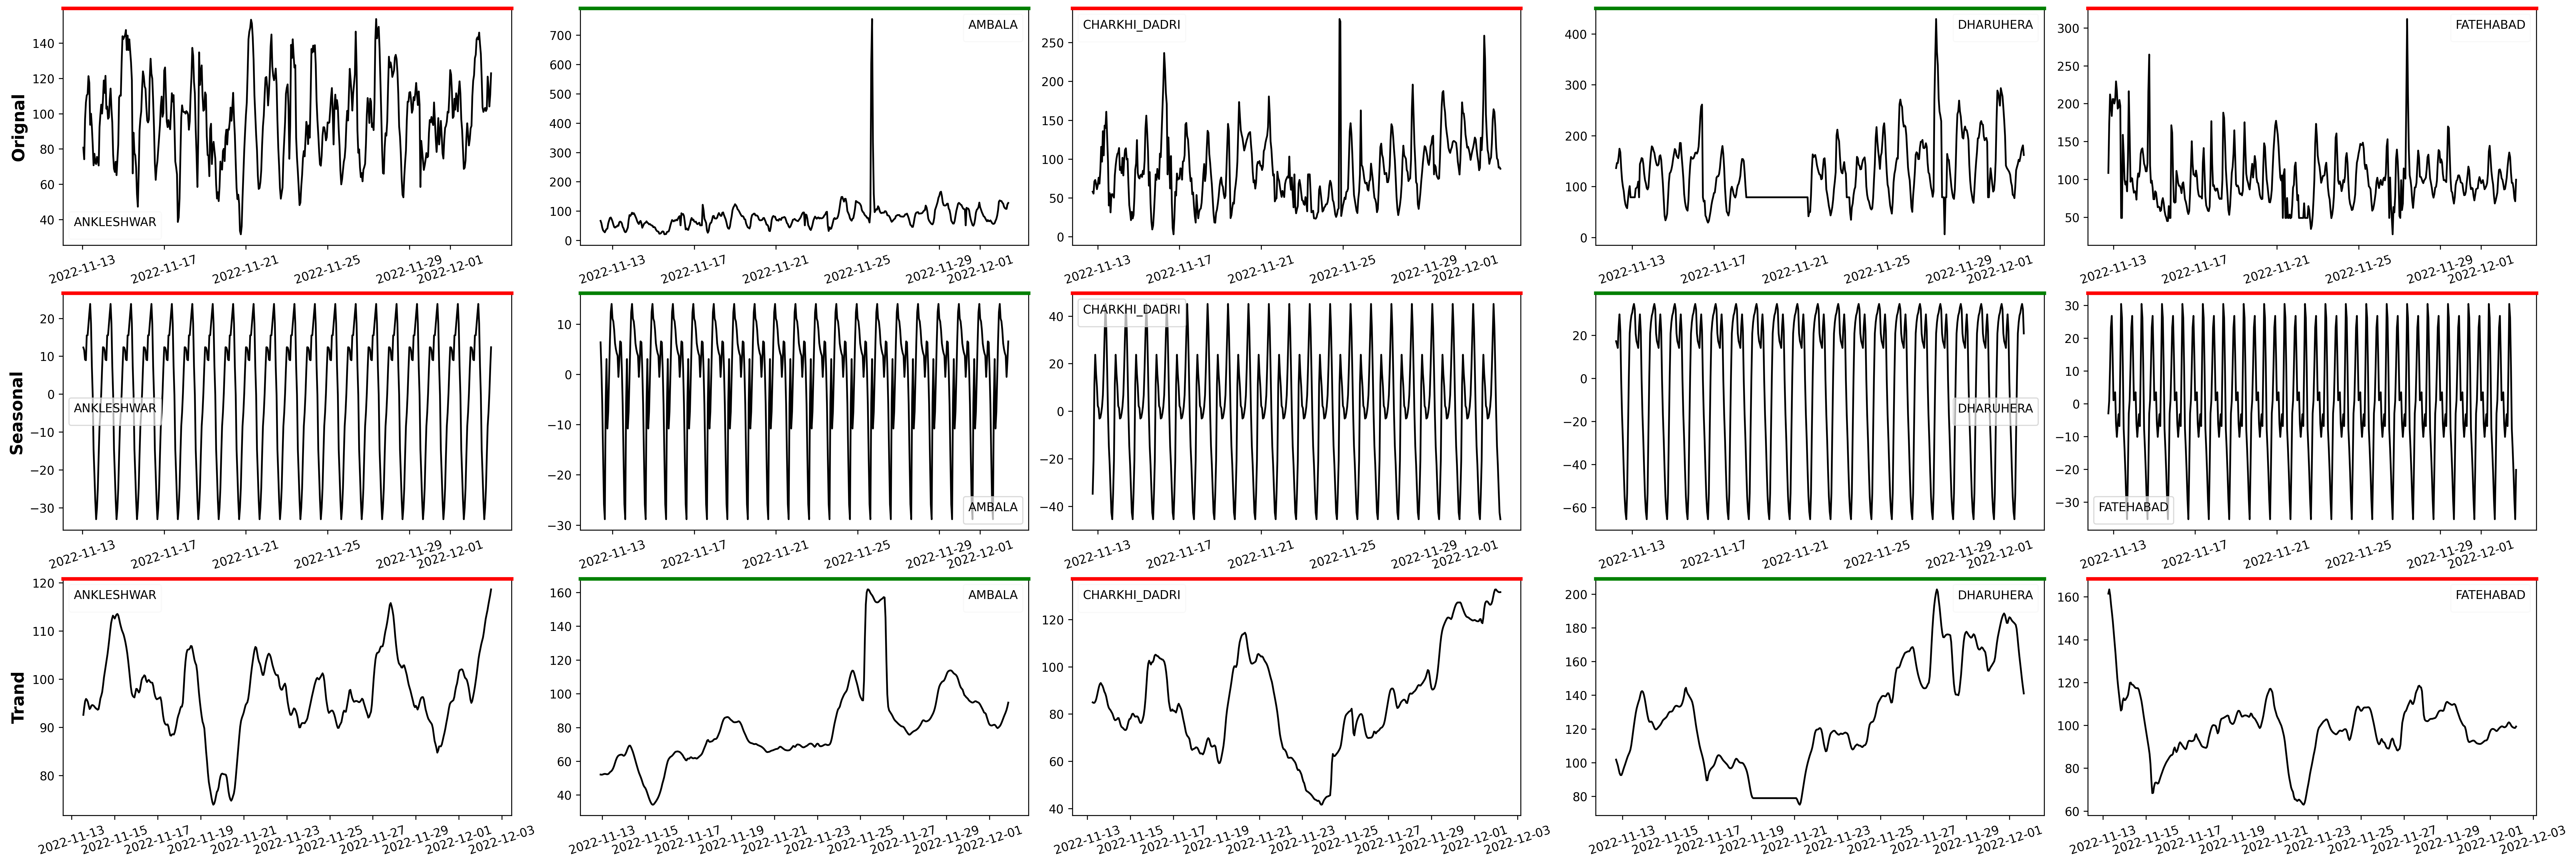
\includegraphics[scale=.3]{1.png}
          \caption{Flowchart of proposed2 (RB-GRU-CNN) model,  where GRU-CNN proposed model may utilize at model learning ($M_i$)}
  	\label{Fig:11}
  \end{figure*}

Workflow can be understood with the following flowchart as shown in Figure 6. The data is cleaned and all the null values are removed. An alpha=0.05 statistical test called the Friedman test is applied. Searches involving ECG,  DL and Artificial Intelligence are performed in conjunction to maximize sensitivity. The following criteria were used for inclusion with the following conditions: 1) Authentic DL studies involving ECG investigations. 2)A well-defined ECG dataset and a detailed description of DL techniques. There were exclusions if studies did not use DL with ECG dataset. The type of DL technique and results in form of error are extracted from each article.


The ability of DL models to predict ECG with minimum errors is studied. Individually applied base models like CNN, RNN, GRU, LSTM and BiLSTM. Single lead- 2  Datasets taken from Physionet website are cleaned and preprocessed. Stationarity of the dataset is checked to stationarize our datasets. Further our data is split into training and testing set. The 80\% data is used for training purpose and the rest 20\% for testing purpose. Although training and testing has been checked with various splittings just to try understand and make sure that no feature completely lies inside a single split. Same features have to be present in both training and testing sets just so our model catches the right references in order to predict. That being told is a major reason behind our model overfitting.
Further we fed this data individually to basic models and ran 20 iterations per data per model. Amongst these 20 iterations the predictions corresponding to the best The Root Mean Squared Error (RMSE) is stored. A final table corresponding to these performance metric is being made by taking mean of individually ran tables on multiple iterations. Researcher also performed a calculative test for deciding with how much percentile  proposed model is working better than basic models on all performance measures whose equations are given in (equation 17, equation 18, equation 19 and equation 20).


(RMSE),  Mean Squared Error(MSE),  Mean Absolute Error(MAE) and Mean Absolute Percent Error(MAPE) is defined as follows:

\begin{equation}
  {RMSE} = \sqrt{\frac{1}{m}\sum_{t=1}^{m}(x_t - \hat{y}_{t}^f)^2}
\end{equation}

\begin{equation}
  {MSE} = \frac{1}{m} \sum_{t=1}^{m} (x_t - \hat{y}_{t}^f)^2
\end{equation}
\begin{equation}
  {MAE} = \frac{1}{m} \sum_{t=1}^{m} \left|x_t - \hat{y}_{t}^f\right|
\end{equation}
\begin{equation}
  {MAPE} =\frac{100}{m} \sum_{t=1}^{m} \left| \frac{x_t - \hat{y}_{t}^f}{x_t} \right|
\end{equation}

where:
\begin{itemize}
  \item $m$ is the total number of data points, 
  \item $x_t$ is the true (observed) value for the $t$-th data point,  and
  \item $\hat{y}_{t}^f$ is the predicted value for the $t$-th data point.
\end{itemize}


Essentially, the RMSE is a commonly used statistic for calculating the average size of errors between predicted and actual values in a model. The square root of the average of the squared discrepancies between predicted and actual values is used to calculate it. RMSE weights greater errors more heavily,  making it susceptible to outliers. The average squared difference between predicted and actual values in a model is measured by MSE. The average of the squared discrepancies between predicted and actual values is used to calculate it. The average absolute difference between predicted and actual values in a model is measured by MAE. When compared to RMSE and MSE,  it is less sensitive to outliers because it handles all errors equally. MAPE is a metric for calculating a method's \% accuracy. It computes the average percentage difference between expected and actual values in relation to the predicted values. 








Several commonly used neural networks were used as contrast models to evaluate the performance and stability of the GRU-CNN model,  including the CNN,  GRU,  LSTM ,  BiLSTM ,  and RNN. In CNN,  GRU,  LSTM,  BiLSTM and RNN models,  the parameters were obtained from the training datasets and tested on the test dataset. A loss function provides a value for the degree of learning when used to evaluate if a prediction model is well trained and learned. Cross entropy,  which defines the separation among two probability distributions,  represents the loss function.
When the cross entropy is low,  the two probability distributions are more close. The formula for cross-entropy is shown below in (eq 21) :

\begin{equation}
  {Loss} =- \frac{1}{m} \sum_{t=1}^{m} \left( x_t \log(\hat{y}_{t}^f) + (1 - x_t) \log(1 - \hat{y}_{t}^f) \right)
\end{equation}

where $m$ is the number of data points,  $x_t$ is the true label (ground truth) of the $t$-th data point,  and $\hat{y}_{t}^f$ is the predicted probability (output) of the $t$-th data point belonging to the positive class.
Training sets fit better when loss values are closer to zero.
It can be see from loss plot Figure 7 that loss values for the chosen models are very close to zero. \\ Now that model is trained,  testing is being performed on unseen 20\% data. Then prediction errors are calculated based on testing performance.

  \begin{figure*}[h!]
   \centering
   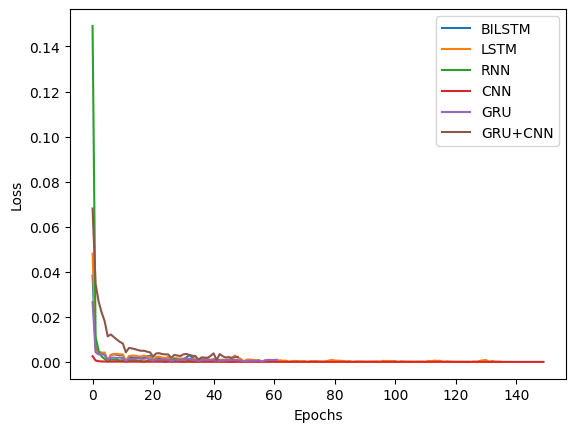
\includegraphics[scale=.5]{val_loss.png}
    \caption{Training losses of BiLSTM, LSTM, RNN, CNN, GRU \& Proposed GRU-CNN models corresponding to the epochs}
    \label{Fig:12}
  \end{figure*}



Proposed-1 has been shown to perform better than the other basic DL models in terms of RMSE, MSE, MAE \& MAPE.  Also discovered is \%imp, which indicates what percentage of the proposed model (Proposed 1) outperforms the implemented classical DL models.


The percentage improvement in RMSE is calculated as:
\begin{equation}
    \text{RMSE}_{\%imp} = \frac{\text{M(i)}_{\text{RMSE}} - \text{Proposed}_{\text{RMSE}}}{\text{M(i)}_{\text{RMSE}}/100}
\end{equation}

where $\text{M(i)}_{\text{RMSE}}$ is the basic model's RMSE,  and $\text{Proposed}_{\text{RMSE}}$ is the RMSE of proposed Model. `\\`

The percentage improvement in MSE is calculated as:
\begin{equation}
    \text{MSE}_{\%imp} = \frac{\text{M(i)}_{\text{MSE}} - \text{Proposed}_{\text{MSE}}}{\text{M(i)}_{\text{MSE}}/100}
\end{equation}

where $\text{M(i)}_{\text{MSE}}$ is the basic model's MSE,  and $\text{Proposed}_{\text{MSE}}$ is the MSE of proposed model. `\\`

The percentage improvement in MAE is calculated as:
\begin{equation}
    \text{MAE}_{\%imp} = \frac{\text{M(i)}_{\text{MAE}} - \text{Proposed}_{\text{MAE}}}{\text{M(i)}_{\text{MAE}}/100}
\end{equation}

where $\text{M(i)}_{\text{MAE}}$ is the basic model's MAE,  and $\text{Proposed}_{\text{MAE}}$ is the MAE of proposed model. `\\`

The percentage improvement in MAPE is calculated as:
\begin{equation}
   \text{MAPE}_{\%imp} = \frac{\text{M(i)}_{\text{MAPE}} - \text{Proposed}_{\text{MAPE}}}{\text{M(i)}_{\text{MAPE}}/100}
\end{equation}

where $\text{M(i)}_{\text{MAPE}}$ is the basic model's MAPE,  and $\text{Proposed}_{\text{MAPE}}$ is the MAPE of proposed model.




